\chapter{SCI-HI Data Analysis}\label{Ch:Data}

\section{Preparing the Data}

Before the data can be analyzed for potential signals, it first has to go through an analysis pipeline to remove noise and make the datasets easier to handle. 

\begin{figure}[htb]
\begin{center}
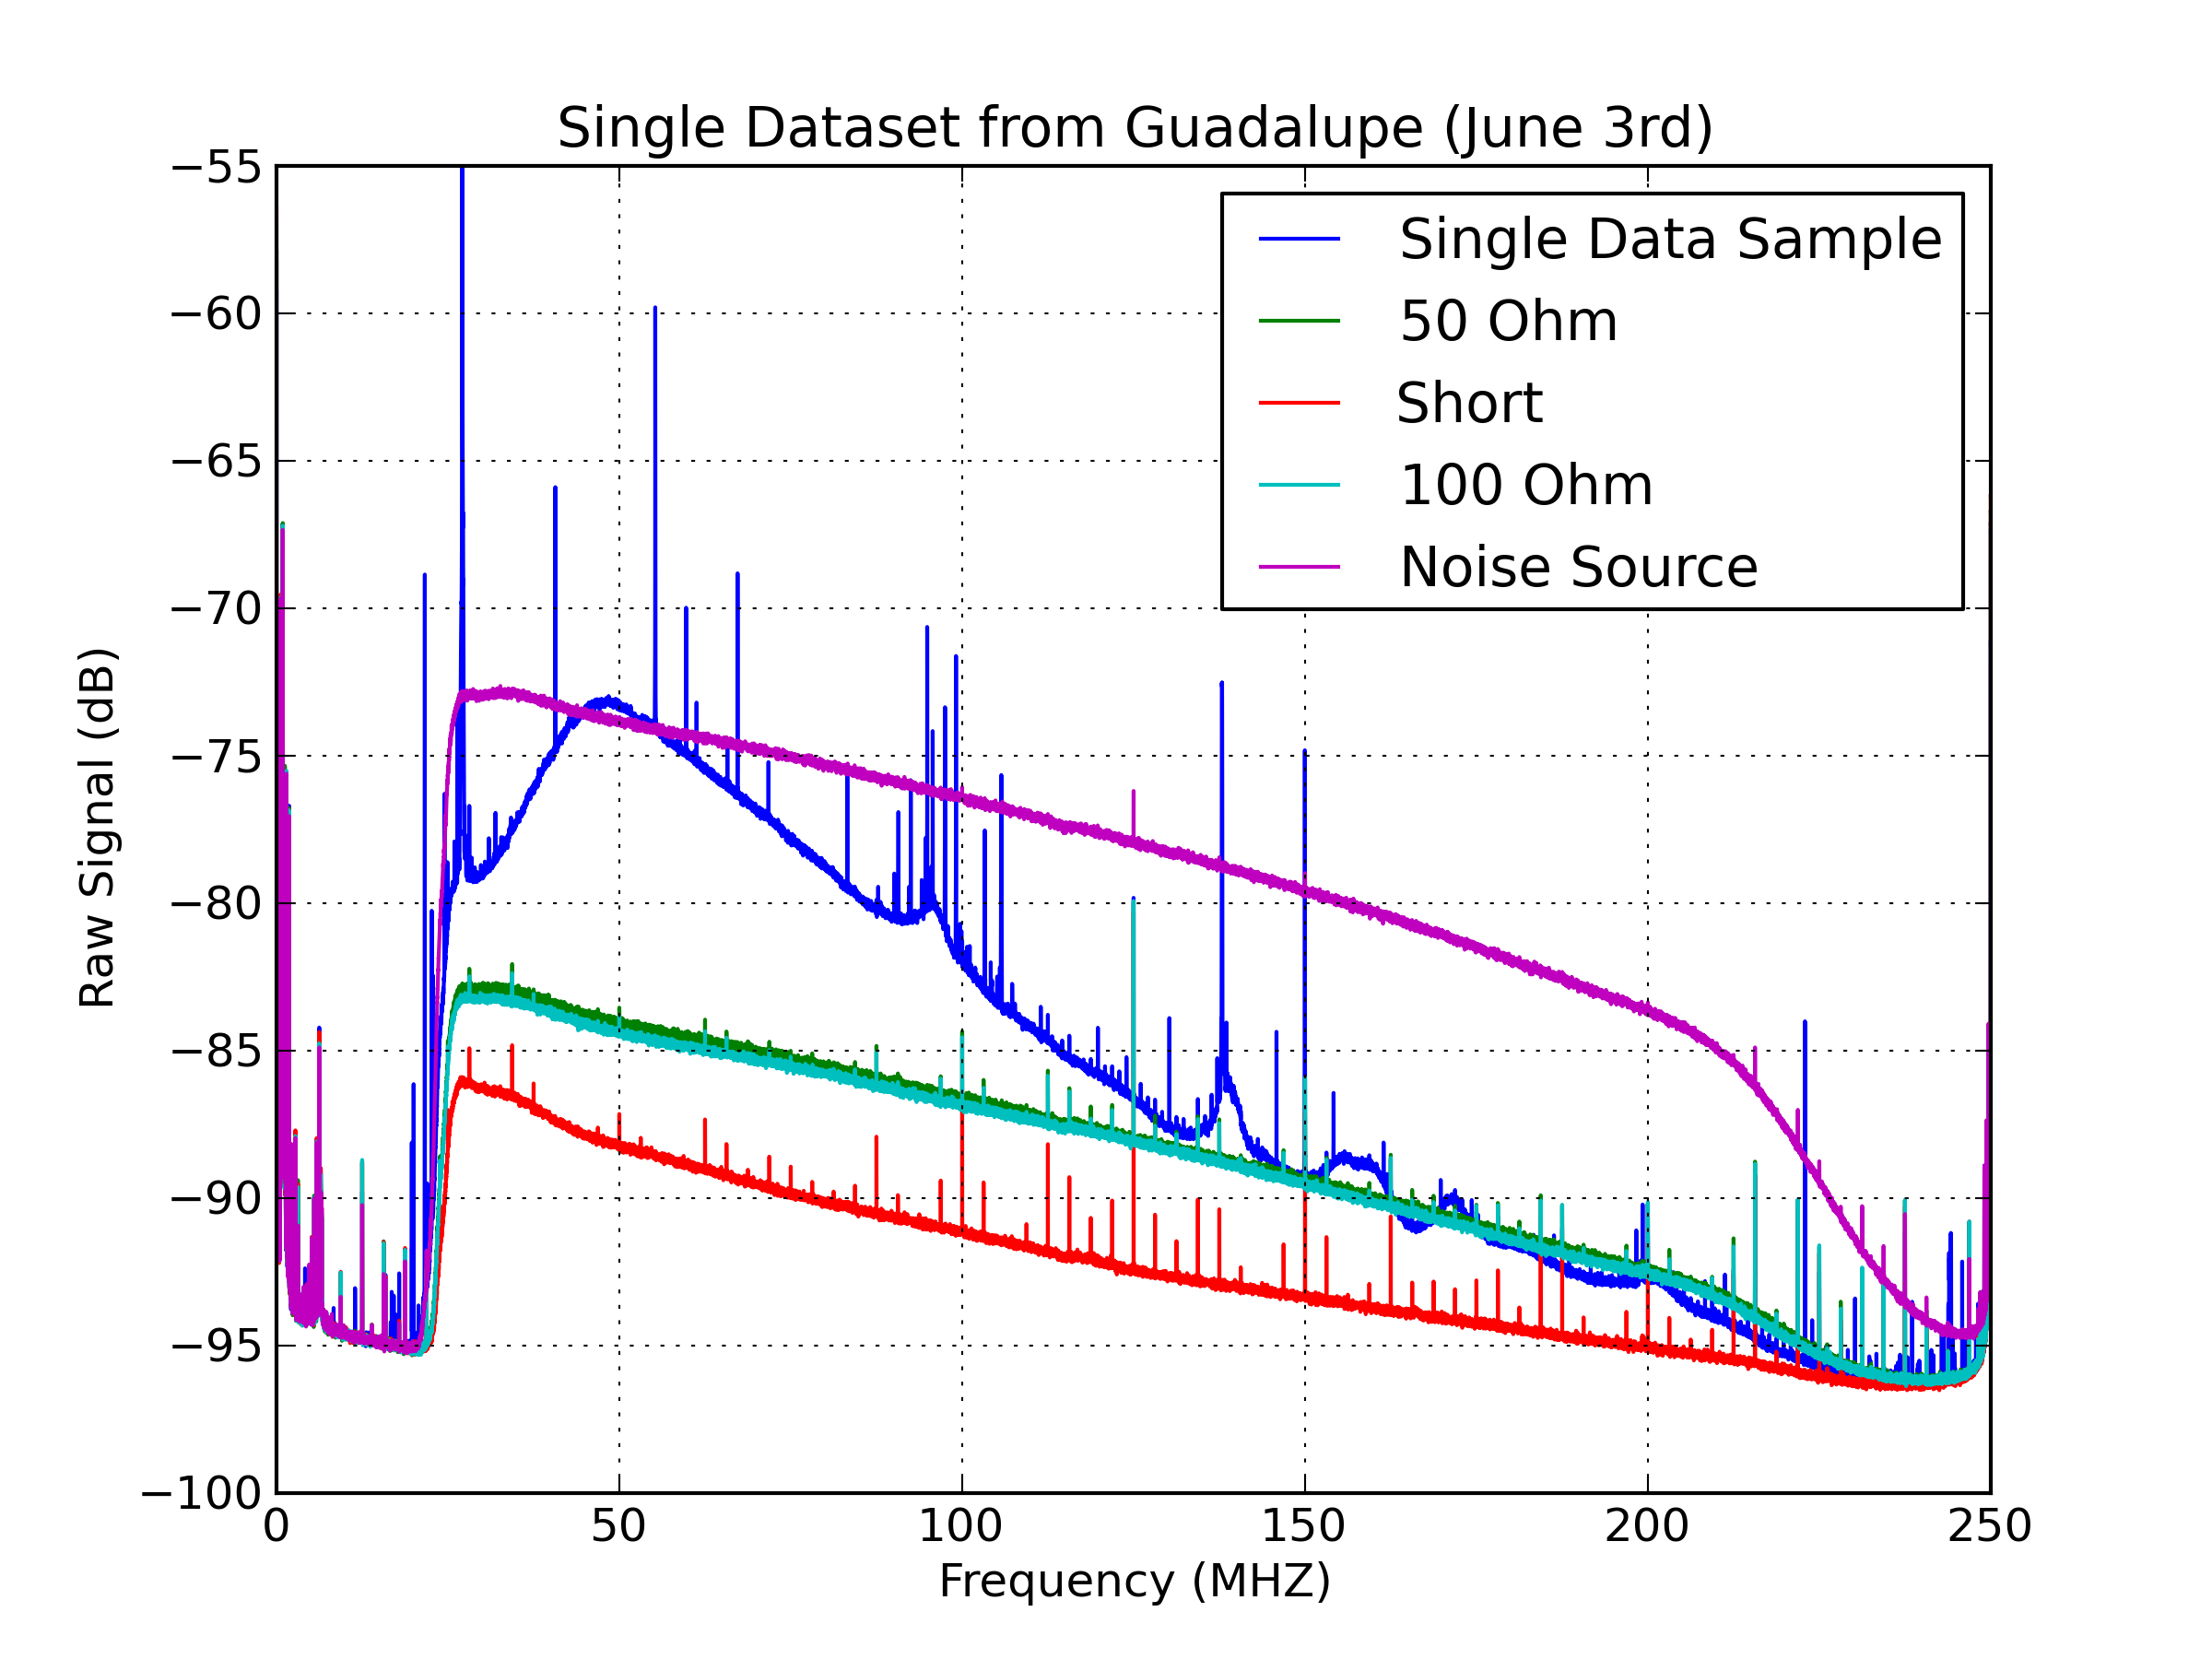
\includegraphics[width=0.9\linewidth]{Data_analysis/figures/single_raw_guad_june03.png}
\caption{Single dataset of the entire frequency spectrum of raw data from the SCI-HI system. Also present are single datasets from the different calibration sources.}
\label{Fig:raw_data}
\end{center}
\end{figure}

\subsection{Integration and Sampling}\label{Sec:int}

The frequency spectrum collected for each second of data is stored in a single file with a header containing some basic information like the timestamp, DC voltage level (when measuring with DC Power Supply), computer temperature, and switch position (antenna vs calibration sources). The spectrum has a bandwidth of 250 MHz, with a frequency resolution of $\sim 7.63$ kHz (or 32769 samples). The data is in units of power (dB) as set by the data processing software. \textcolor{red}{I know there's something that Jose does to set these units but I'm not sure exactly what it is.} 

An example of the data collected by the system is shown in Figure \ref{Fig:raw_data}. Also included is a single sample of data from each of the calibration sources (Short, 50 $\Omega$, 100 $\Omega$, and Noise Source). The sharp signal cutoffs at 30 MHz and 200 MHz are from the high and low pass filters in the system.

\begin{figure}[htb]
\begin{center}
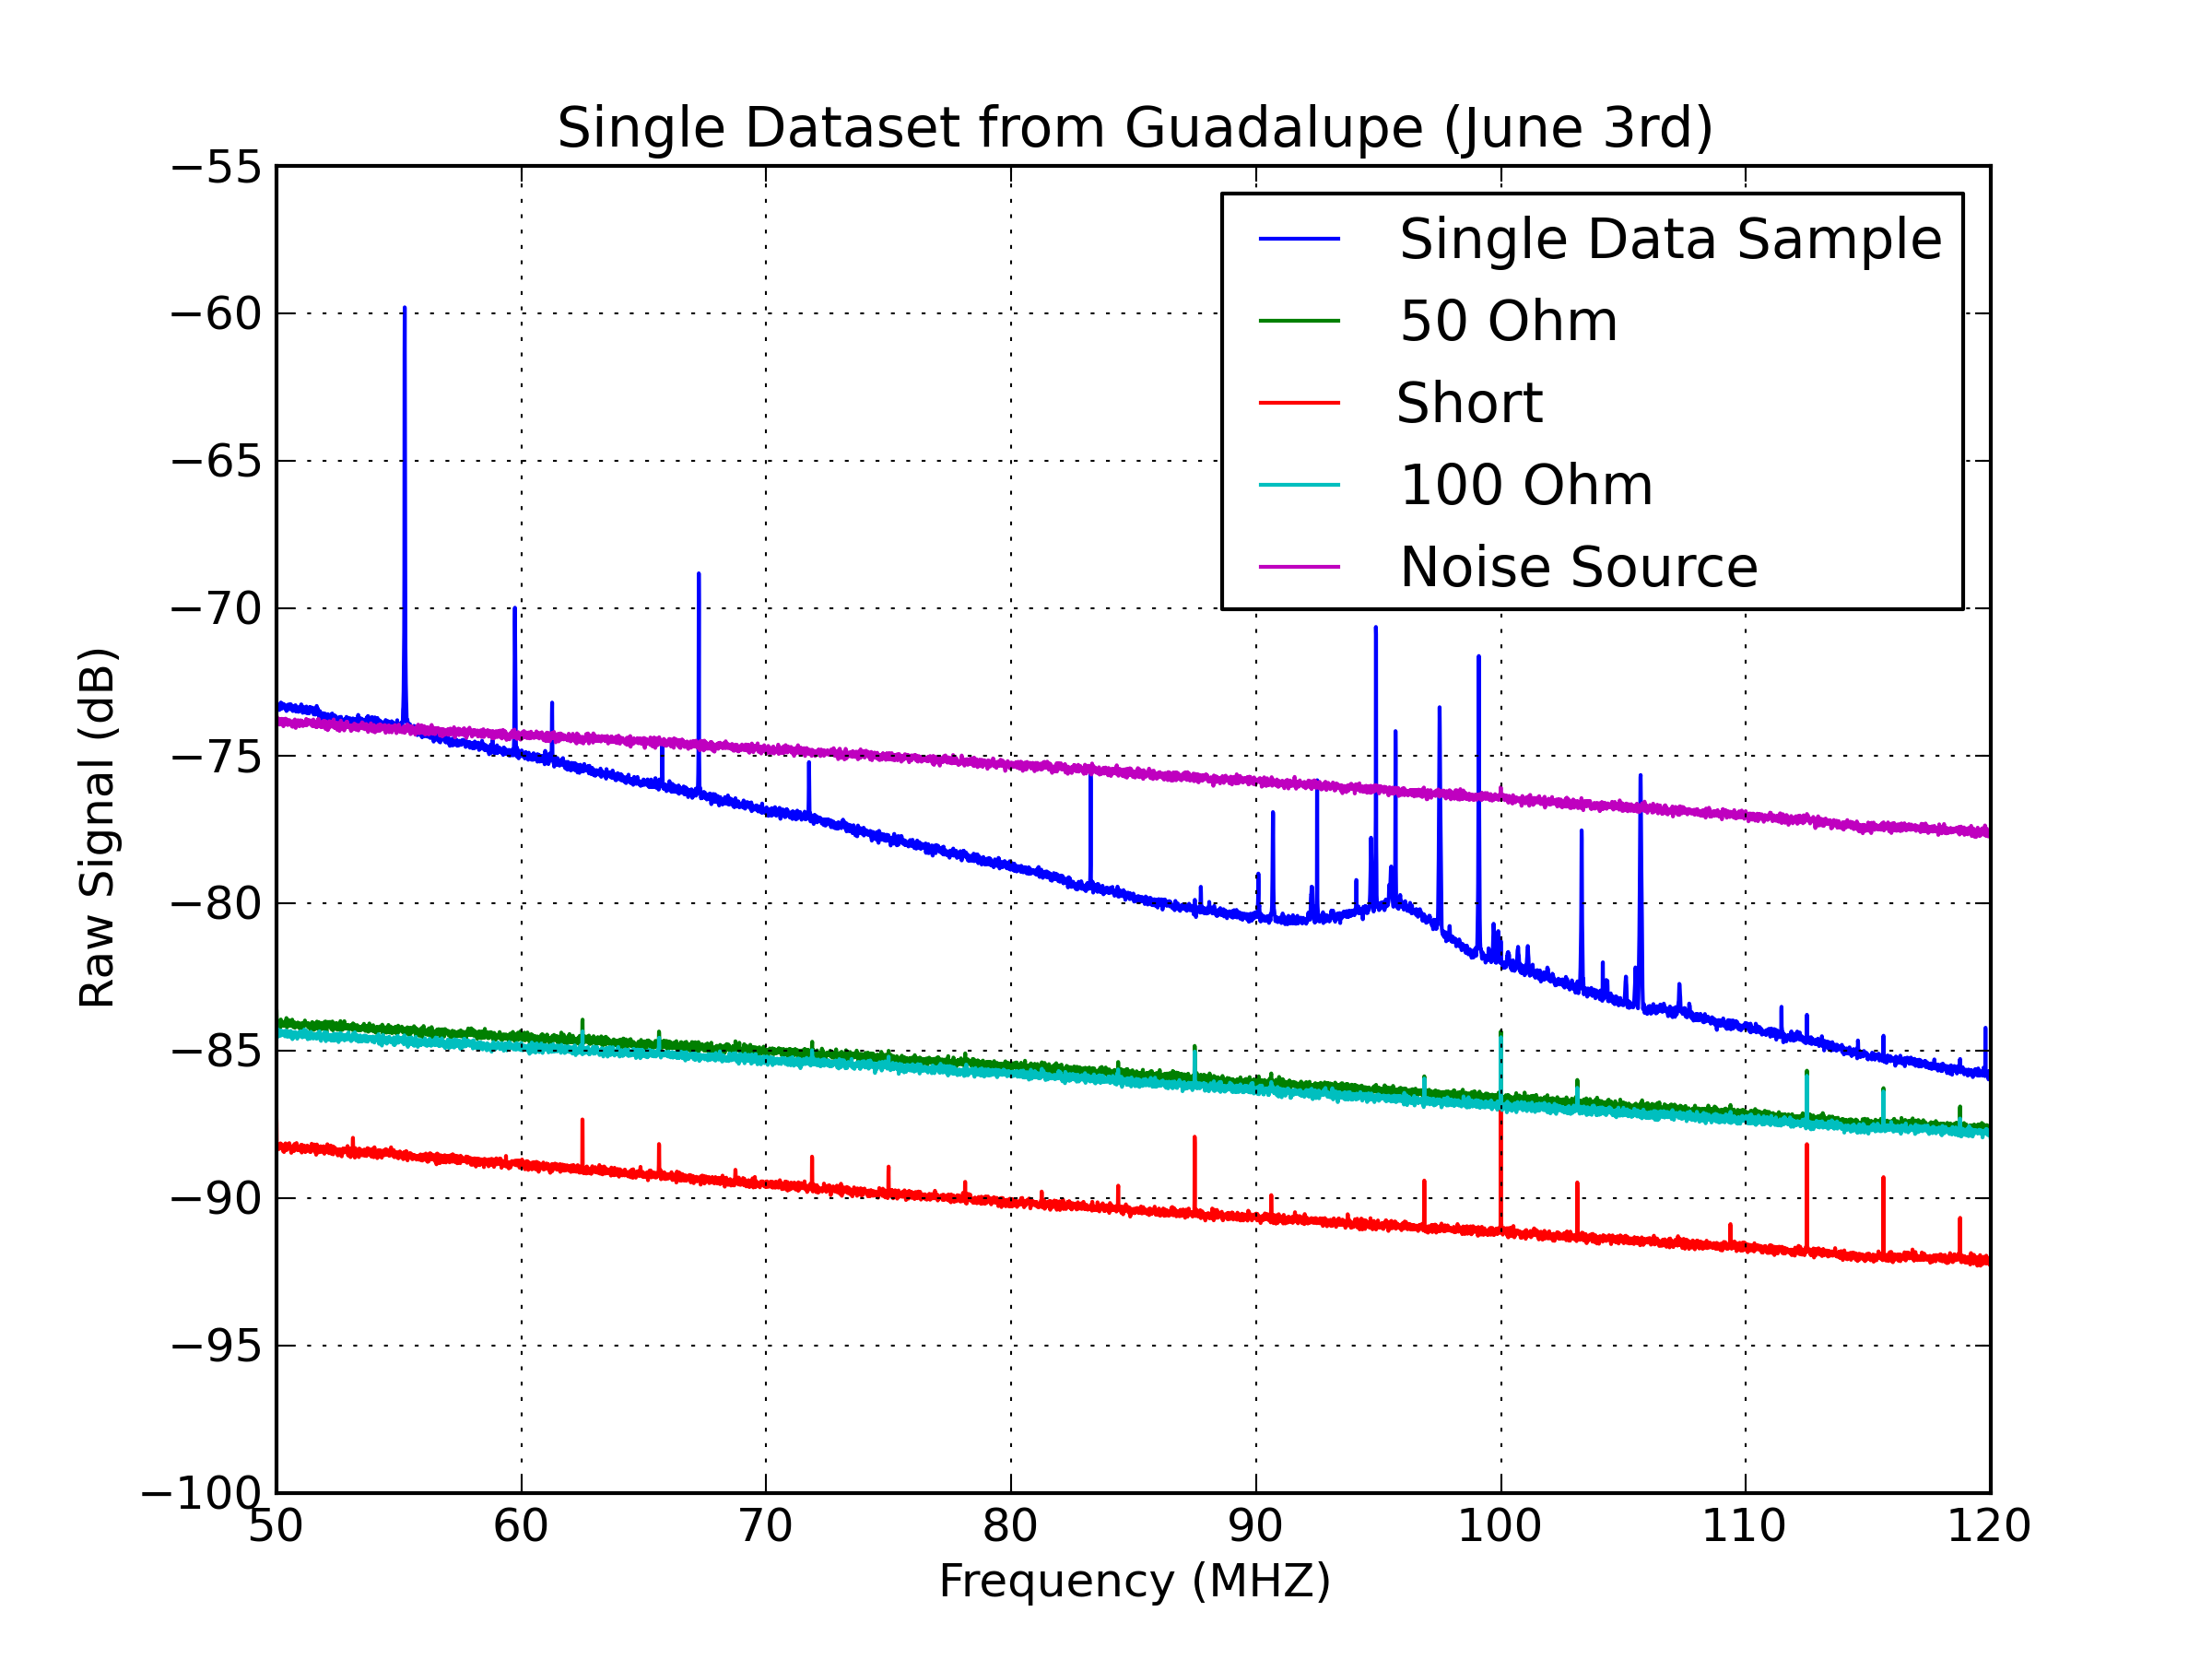
\includegraphics[width=0.9\linewidth]{Data_analysis/figures/single_raw_trunc_guad_june03.png}
\caption{Single dataset of a truncated spectrum of raw data from the SCI-HI system. Also present are single datasets from the different calibration sources.}
\label{Fig:raw_data_trunc}
\end{center}
\end{figure}

\subsection{Truncation}

Because the data we are interested in is a subset of the overall spectrum, one of the first things that we can do is to truncate frequency range of the data to make it smaller. For example, plotting the key frequency range for the SCI-HI data as collected in 2013 (50-120 MHz) helps us to pick out some of the things going on that are harder to see in the full spectrum (see Figure \ref{Fig:raw_data_trunc}). 

In the truncated dataset, it is easier to identify significant features in the data. For example, the nearly linear slope of the signal helps us confirm that the antenna is seeing the spectrum from the Milky Way Galaxy, while the excess of noise in the FM band and the bump in the middle of the FM band are evidence of RFI (both external and self-generated). 

\subsection{RFI Excision}

Another early stage of the pipeline is RFI excision (both in frequency and time). 

\subsubsection{RFI Frequency Flagger}

RFI excision in frequency is done using a flagger that does a threshold cut for each dataset. Because the data is expected to have a polynomial fit, the first step is to fit a two term polynomial to a small subset of the data (center frequency plus a its nearest neighbors). The subset of data is then divided by the polynomial and a mean and variance of the flattened data is calculated. If the data point at the center frequency is further from the mean than a set threshold, then that data point is flagged. 

The exact threshold and number of neighbors used to set the mean can be tweaked, but the typical values I used were a 3$\sigma$ threshold and 32 neighbors on either side. If a data point is flagged, it is masked out of the data and will not be included in the data in the future. 

\begin{figure}[htb]
\begin{center}
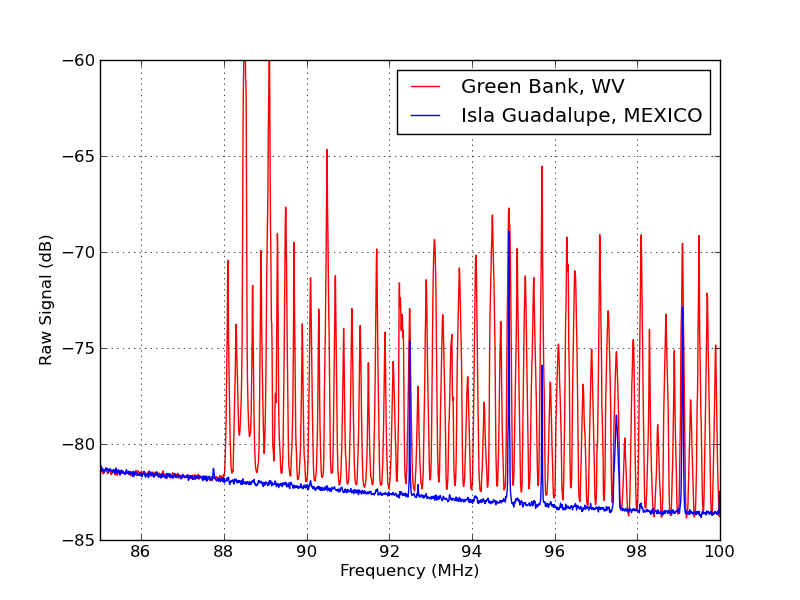
\includegraphics[width=0.9\linewidth]{Data_analysis/figures/FM_band_comp.png}
\caption{RFI comparison in the FM band between Isla Guadalupe and Green Bank, West Virginia. }
\label{Fig:FM_band}
\end{center}
\end{figure}

\subsubsection{RFI in the FM Band}

One of the frequency bands where RFI excision is particulary challenging is in the FM band (88-108 MHz). In this band, the variance of the signal can be quite large; making the RFI excision procedure less reliable. For many of our testing sites like Green Bank, WV the entire FM band is occupied with large RFI signals (as discussed in Chapter \ref{Ch:RFI}). This can be seen in Figure \ref{Fig:FM_band}, where the RFI signals are on average $\sim$10 dB above the floor. 

On the other hand, the FM band RFI signals from Isla Guadalupe are mostly $\leq$1 dB. These RFI signals are small enough to be missed by the RFI flagger and may be run through the rest of the pipeline stages. The few large spikes $\geq$5 dB above the floor will be removed by the RFI excision code. 

\subsubsection{Time-variable RFI}

While most of the RFI in the data is time independent and can be flagged out in each dataset indpendently, some of the RFI has a strong time-dependence. 

\paragraph{Time-variability of RFI due to Meteor Scatter}

Meteoroids are always passing through Earth's atmosphere. These meteoroids have a wide spectrum of sizes starting from $\leq$10 nm. As these meteoroids pass through the earth's atmosphere, some of their atoms are vaporized. Inelastic collisions between these atoms and air molecules in the atmosphere can lead to ionization \cite{meteor_review}. 

The result of this ionoization is a thickening of the Earth's ionosphere along the meteor trail, causing the ionosphere to become opaque to shorter wavelength photons along the trail. This opacity extends the range of signals such as FM radio to more distant locations than would normally be accessible.

In the SCI-HI data, this leads to a time-variable increase in the FM band RFI. For short time periods the strength of RFI signals from FM radio towers becomes larger. The duration of these signals is relatively small \textcolor{red}{(Add an estimate from our data based on the width of these events?)}, diminishing as free electrons diffuse away from the original meteor trail. 

\textcolor{red}{Add a plot here that shows a short time sample of RFI increase due to meteor scatter.}

\paragraph{Time-variability of RFI from Local Sources}

Another source of time-variable RFI is local noise from the surroundings. Our site at Isla Guadalupe was a few km from the local fishing village, which meant that occasionally RFI was picked up from the village when the diesel generator was powered on during the day. Additionally, the site was a few hundred meters from the road that led from the village to the rest of the island. When vehicles drove past the site (a few times each day), RFI from the vehicles such as broad band RF from spark plugs could be seen in the data. 

\subsubsection{Time-variable RFI Flagging}

In order to remove such time-variable RFI, I wrote a second RFI flagger identical to the frequency flagger, except that it works along the time axis. I typically used the same threshold and number of neighbors as the frequency flagger. 

\subsection{Rebinning}

Because the data is collected at a much higher resolution than is needed for the analysis, it needs to be rebinned to lower resolution. This can be done either in frequency or time. Compression is done after RFI flagging in order to keep a single $''$bad$''$ channel from affecting the overall signal. The mean of the unflagged data for a given bin scale becomes the new data point. In addition, a new data point is left as a flagged point if over half of the data used to make it were flagged. 

\section{Calibrating the Data}

After RFI removal and compression, the data is ready for calibration. Calibration is used both to put the data into correct units and also remove artificial structure in the frequency spectra. 

\subsection{Calibration Datasets}

Part of the SCI-HI system, as laid out in Chapter \ref{Ch:System}, is an electro-mechanical switch that allows data collection from both the antenna and known temperature sources placed on the different switch input terminals. Figures \ref{Fig:raw_data} and \ref{Fig:raw_data_trunc} show the different datasets measured with the system, which are also known as $''$Johnson Noise$''$ datasets. 

In these datasets, the temperature of each source can be separated into different terms. 

\paragraph{Short Terminator}
For the $''$Short$''$ signal, a shorting terminator is placed on the switch input terminal. This means that all of the signal seen in the data processor is coming from the SCI-HI system. This includes both instrumental noise and thermal noise, and we'll call this temperature $T_{short}$.

\paragraph{$50 \Omega$ Terminator}
For the $'' 50 \Omega ''$ signal, a load is placed on the switch input with an impedance of $50 \Omega$. The load provides an input of the current ambient temperature, and instrumental and termal noise adds additional signal. There is an another noise term ($T_Z$), which depends on the match between the impedence of the first stage amplifier and the load. So, we can write the $50 \Omega$ temperature as:

\begin{equation}
T_{50 \Omega} = T_{amb}+T_{Z50}+T_{short}
\end{equation}

\paragraph{$100 \Omega$ Terminator}
For the $'' 100 \Omega ''$ signal, a load is placed on the switch input with an impedance of $100 \Omega$. This load provides a nearly identical temperature as the $50 \Omega$ load, with the exception of the impedance term. So, we can write the $100 \Omega$ temperature as:

\begin{equation}
T_{100 \Omega} = T_{amb}+T_{Z100}+T_{short}
\end{equation}

Comparing $T_{50 \Omega}$ and $T_{100 \Omega}$ allows us to determine the significance of the impedance term. In Figure \ref{Fig:raw_data}, we see that the two signals are nearly identical. This tells us that the impedance term does not play a significant role in our system noise.

\paragraph{Artificial Noise Source}
For the $''$Noise Source$''$ signal, an artificial noise source with $50 \Omega$ impedance is placed on the switch input. This source provides both an ambient temperature signal and an additional artificial noise signal ($T_{Noise}$) which can be independently measured. The impedance noise term matches the $50 \Omega$ impedance term. So, we can write the noise source temperature as:

\begin{equation}
T_{NS} = T_{Noise} + T_{amb}+T_{Z50}+T_{short}
\end{equation}


\paragraph{Antenna}
For the signal from the HIbiscus antenna, we can write a similar equation for the temperature. In this case, we have thermal and instrument noise and an impedance term, as well as signals from the sky. 

\begin{equation}\label{Eq:T_ant}
T_{Ant} = T_{sky}+T_{Zant}+T_{short}
\end{equation}

\subsection{On-site Impedance}
Impedance can be measured using a Vector Network Analyzer (VNA) looking at the reflectivity (S11) data for the input sources. The calibration sources have an impedance that is constant in frequency ($50 \Omega$ or $100 \Omega$) and has no phase.

In comparison, the HIbiscus antenna has a complex impedance that varies with frequency and has a phase component (see Section \ref{Sec:HIbiscus_Imp} and Figures \textcolor{red}{Add references here}). This impedance must be measured in-situ, since it can depend on the exact layout of the system and the shape of the terrain around the antenna. 

\begin{figure}[htb]
\begin{center}
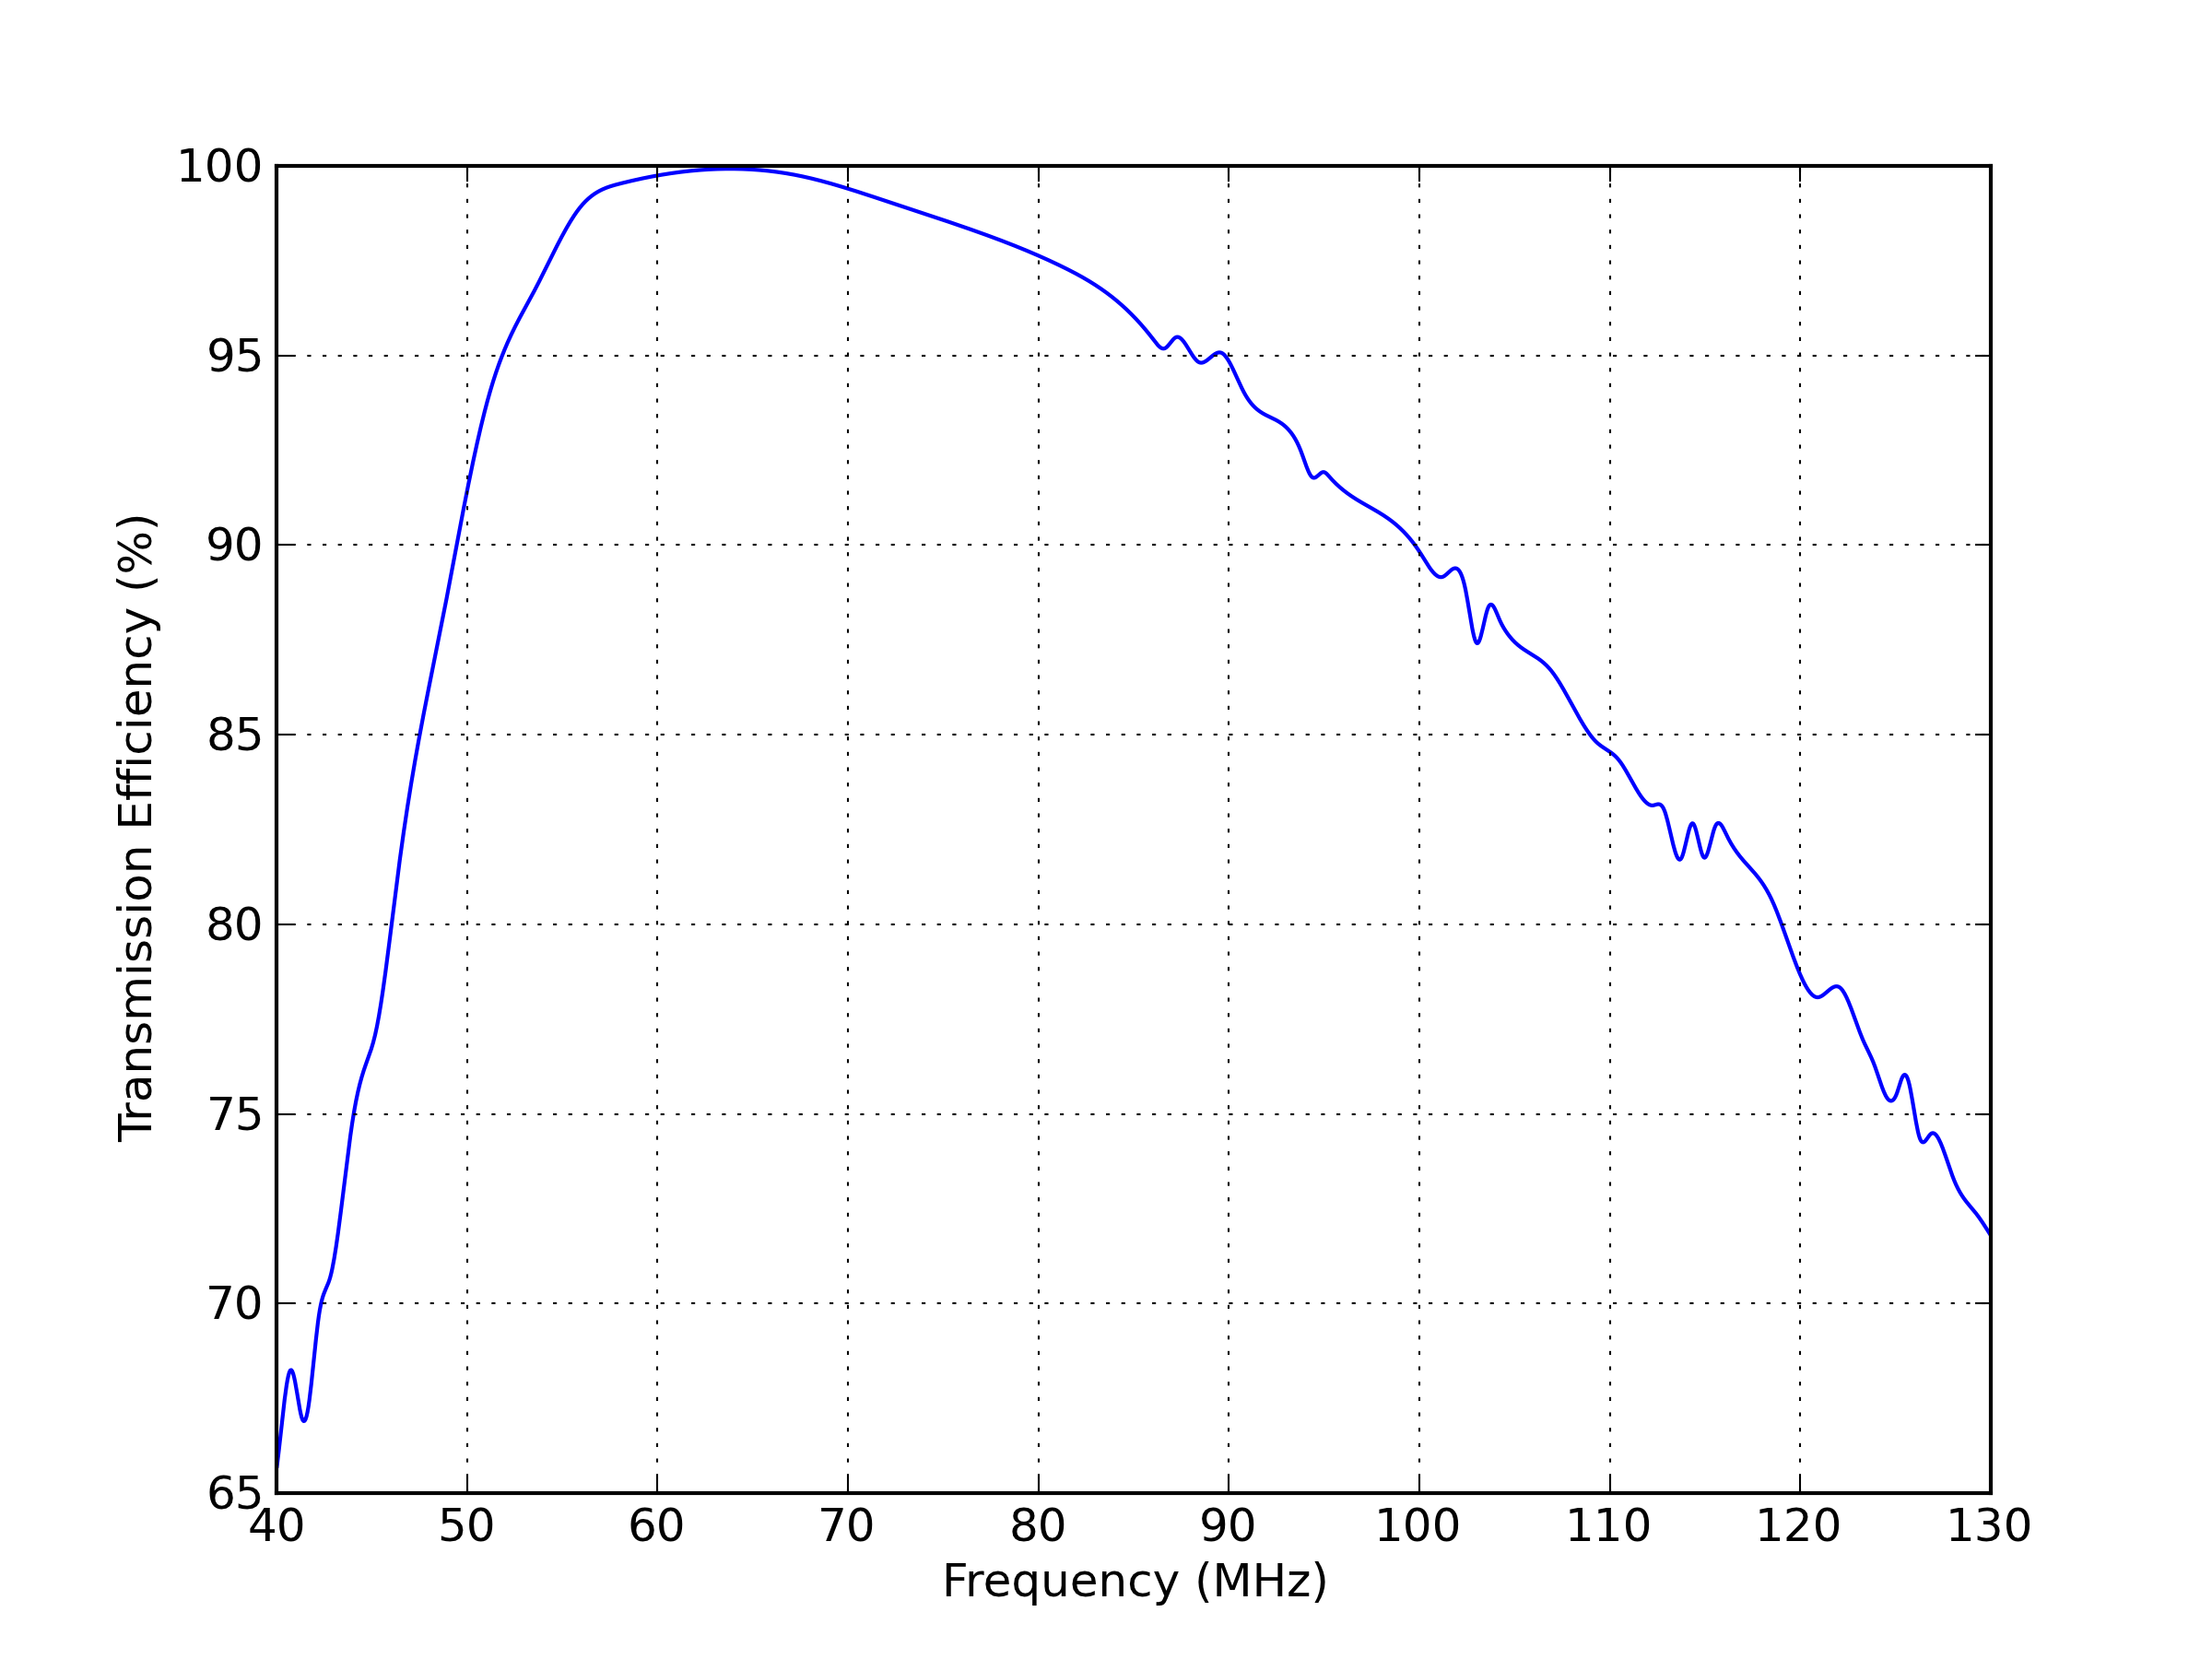
\includegraphics[width=0.9\linewidth]{Data_analysis/figures/old_ant_efficiency.png}
\caption{SCI-HI system transmission efficiency as calculated using S11 measurements of the HIbiscus antenna and first stage amplifier. Here 100 \% efficiency means that all the power from the sky collected by the antenna is seen by the first stage amplifier. }
\label{Fig:eff}
\end{center}
\end{figure}

\subsubsection{Efficiency ($\eta$)}
For the antenna, the $T_{impAnt}$ signal can be calculated using the match between the antenna impedance and the amplifier impedance. Impedance (Z) has a real (R) and imaginary (X) term, each of which vary as a function of frequency ($\nu$) and can be calculated from the S-parameter data: \textcolor{red}{Add a discussion here about how S11 data is compared to a 50 Ohm reference source.}

\begin{equation}
R(\nu) = \frac{50*(1- |S11|^2)}{(1-\Re(S11))^2+\Im(S11)^2}
\end{equation}

\begin{equation}
X(\nu) = \frac{2*50*\Im(S11)}{(1-\Re(S11))^2+\Im(S11)^2}
\end{equation} 

Instead of being a separate term, $T_{Zant}$ can be considered a change to the magnitude of $T_{sky}$ and can be written as a transmission efficiency ($\eta$). This transmission efficiency depends on both the antenna impedance $Z_{ant} = R_{ant}+i X_{ant}$ and amplifier impedance $Z_{amp} = R_{amp} + i X_{amp}$, and is defined by the equation: \textcolor{red}{Add reference for this derivation}

\begin{equation}
\eta (\nu) = \frac{\sqrt{4 |R_{ant}*R_{amp}|}}{(R_{ant}+R_{amp})^2+(X_{ant}+X_{amp})^2}
\end{equation}

For the June 2013 deployment data, the efficiency is shown in Figure \ref{Fig:eff}. With the efficiency, our antenna temperature equation (\ref{Eq:T_ant}) can be re-written as:

\begin{equation}
T_{Ant}(\nu) = \frac{T_{sky}}{\eta} + T_{short}
\end{equation}


\subsection{Milky Way Galaxy (GSM) Modeling}

One of the big challenges of calibration in radio astronomy is figuring out what to use as a known temperature source. For the SCI-HI experiment, the only astronomical source accessible given our $\sim 55 ^\circ$ antenna beam is radio signals from the Milky Way Galaxy. 

\begin{figure}[htb]
\begin{center}
\includegraphics[width=0.9\linewidth]{Data_analysis/figures/beam.pdf}
\caption{Simulated HIbiscus antenna beam on the sky in RA, DEC coordinates at Isla Guadalupe's latitude. Each map corresponds to a different LST at 70 MHz. }
\label{Fig:HIbiscus_beam}
\end{center}
\end{figure}

\subsubsection{HIbiscus Beam Coverage}

Once the SCI-HI system has been set up on-site at a particular location, the Earth rotates as the antenna constantly points towards the zenith. Due to this rotation, the beam of the Hibiscus antenna looks at different parts of the sky at different times of day. 

The exact beam coverage can be calculated using the simulated HIbiscus beam and the site latitude, shown in Figure \ref{Fig:HIbiscus_beam}.  It is important to note that here we use Local Sidereal Time (LST), not Coordinated Universal Time (UTC), because we care about the motion of the Milky Way Galaxy rather than the sun.  

\begin{figure}[htb]
\begin{center}
\includegraphics[width=0.9\linewidth]{Data_analysis/figures/gsm_fig.pdf}
\caption{Sky temperature calculated using the GSM model from de Oliveira-Costa et al \cite{GSM_model} at 70 MHz. The temperature map is in units of $log_{10} Kelvin$, while the map coordinates are in RA, DEC. }
\label{Fig:GSM_model}
\end{center}
\end{figure}

\subsubsection{GSM Model}

The main signal from the sky at 40-130 MHz is the Milky Way Galaxy, which has temperatures of over $1000$ Kelvin for most of the SCI-HI frequency band. However, most of the Milky Way Galaxy signal comes from the plane of the galaxy, which oves from horizon to zenith to horizon due to Earth's rotation. This motion causes the galactic plane to drift in and out of the HIbiscus beam over time. 


The Galactic Global Sky Model (GSM) is the current best model for the sky, including the Milky Way Galaxy, at these frequencies. It is a model created by interpolating data from many different publically available radio surveys with a frequency range of 10 MHz - 100 GHz. The model and software \cite{GSM_model}, can be used to make maps in our frequency band. One such map is shown in Figure \ref{Fig:GSM_model}, displayed using equatorial coordinates (right ascension, RA, and declination, DEC) to match the beam maps. 

\textcolor{red}{Add plot of uncalibrated (dB) data for one day at 70 MHz to show the time dependence here.}

\subsubsection{Expected Sky Signal}

Using the combination of the GSM model and the simulated HIbiscus antenna beam, the beam-averaged sky temperature can be calculated using the following equation: 

\begin{equation}
T_{GSM} (\nu,t) = \frac{ \int d \Omega GSM (\theta, \phi, \nu) \mathcal{B} (\theta - \theta_0(t), \phi - \phi_0(t),\nu)}{\int d\Omega \mathcal{B} (\theta -\theta_0(t), \phi - \phi_0(t), \nu)}
\end{equation}

Where $GSM (\theta, \phi, \nu)$ is the model data and $\mathcal{B} (\theta - \theta_0(t), \phi - \phi_0(t),\nu)$ is the simulated beam, with ($\theta_0 (t),\phi_0 (t)$) being the beam center. 

\subsection{Calibration Factor Calculation}

Although all of our datasets have been described using temperature, the actual signals measured by the system are given in units of power in dB (as discussed in Section \ref{Sec:int}). Therefore, we need to convert our signals from power to temperature. This conversion can be written with a simple calibration factor $K(\nu)$ such that:

\begin{equation}
P(\nu,t) = K(\nu)*T(\nu,t)
\end{equation}

Calculating the calibration factor can be done with either the known source datasets or the Milky Way Galaxy model. 

\subsubsection{Johnson Noise Calibration}

Using the Johnson noise datasets, we can determine a calibration factor $K_{JNC}(\nu)$ using the various datasets. We start with the following four datasets:

\begin{equation}
P_{short} = K_{JNC}*T_{short}
\end{equation}
\begin{equation}
P_{50 \Omega} = K_{JNC}*(T_{amb} + T_{Z50} + T_{short})
\end{equation}
\begin{equation}
P_{100 \Omega} = K_{JNC}*(T_{amb} + T_{Z100}+T_{short})
\end{equation}
\begin{equation}
P_{NS} = K_{JNC}*(T_{Noise}+T_{amb}+T_{Z50}+T_{short})
\end{equation}

By re-arranging the datasets, we can calculate the calibration factor in three ways (depending on what we know the best). 

Version 1:
\begin{equation}
K_{JNC} = \frac{T_{amb}}{P_{50 \Omega} - P_{short}}
\end{equation}

Version 2:
\begin{equation}
K_{JNC} = \frac{T_{amb}}{P_{100 \Omega} - P_{short}}
\end{equation}

Version 3:
\begin{equation}
K_{JNC} = \frac{T_{Noise}}{P_{NS}-P_{50 \Omega}}
\end{equation}

Now, versions 1 or 2 assume that $T_{Z50}$ or $T_{Z100}$ are very small and we know $T_{amb}$, while version 3 assumes that we know $T_{Noise}$ very well.

In all of these versions, we need to remove the thermal noise component before using the data for calibration. The way that we do this is to take the average of many calibration datasets and then fit the average to a simple 2 parameter power law in frequency. 

\textcolor{red}{Make plots of each of the four averaged datasets + their fit for one day.}

\textcolor{red}{Add further discussion of how we looked at the data and tried to model $T_{Z*}$, and why we couldn't use the Noise Source because we couldn't find precise enough values for the noise temperature as a function of frequency.}

We used a calibration strategy corresponding to version 1 for our calibration, with $T_{amb} = 300 Kelvin$ as a constant, and assuming that $T_{Z50}=0$. 

\begin{figure}[htb]
\begin{center}
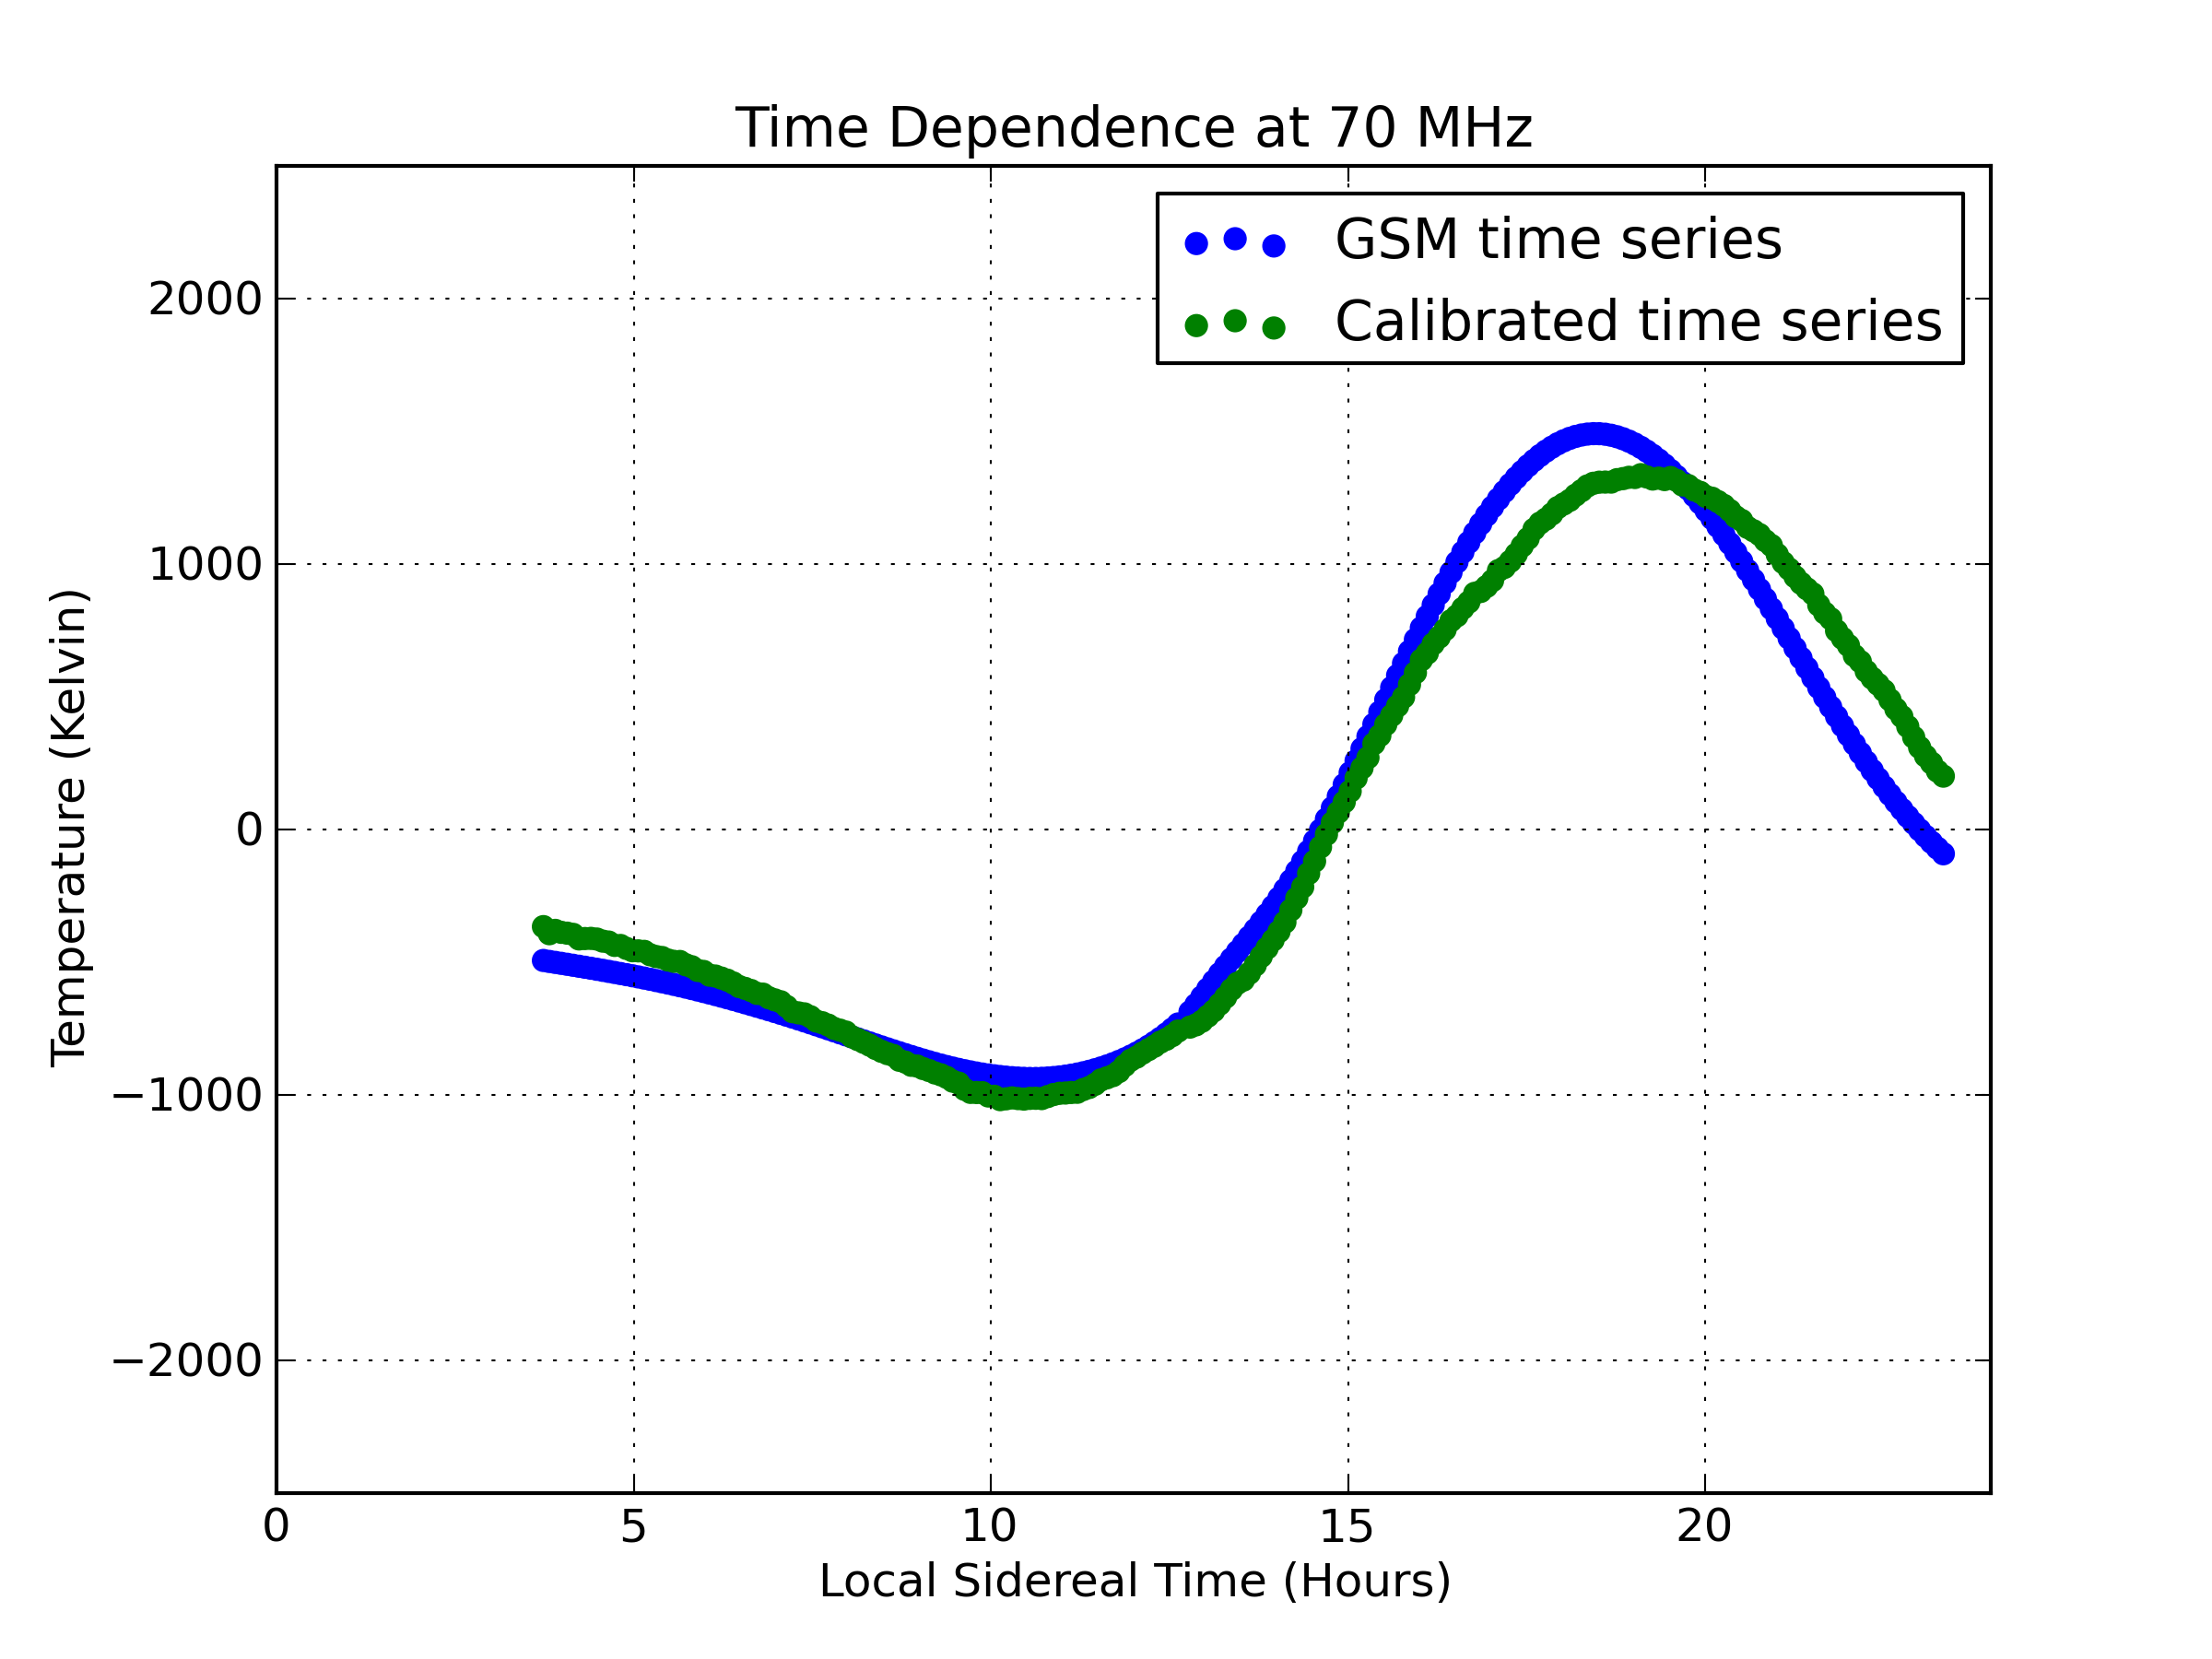
\includegraphics[width=0.95\linewidth]{Data_analysis/figures/June_06_K_dgsm_time_series.png}
\caption{Single day fit of the $K_{\Delta GSM}$ calibration term with data collected on June 6th, 2013 at 70 MHz. }
\label{Fig:Kdgsm}
\end{center}
\end{figure}

\begin{figure}[htb]
\begin{center}
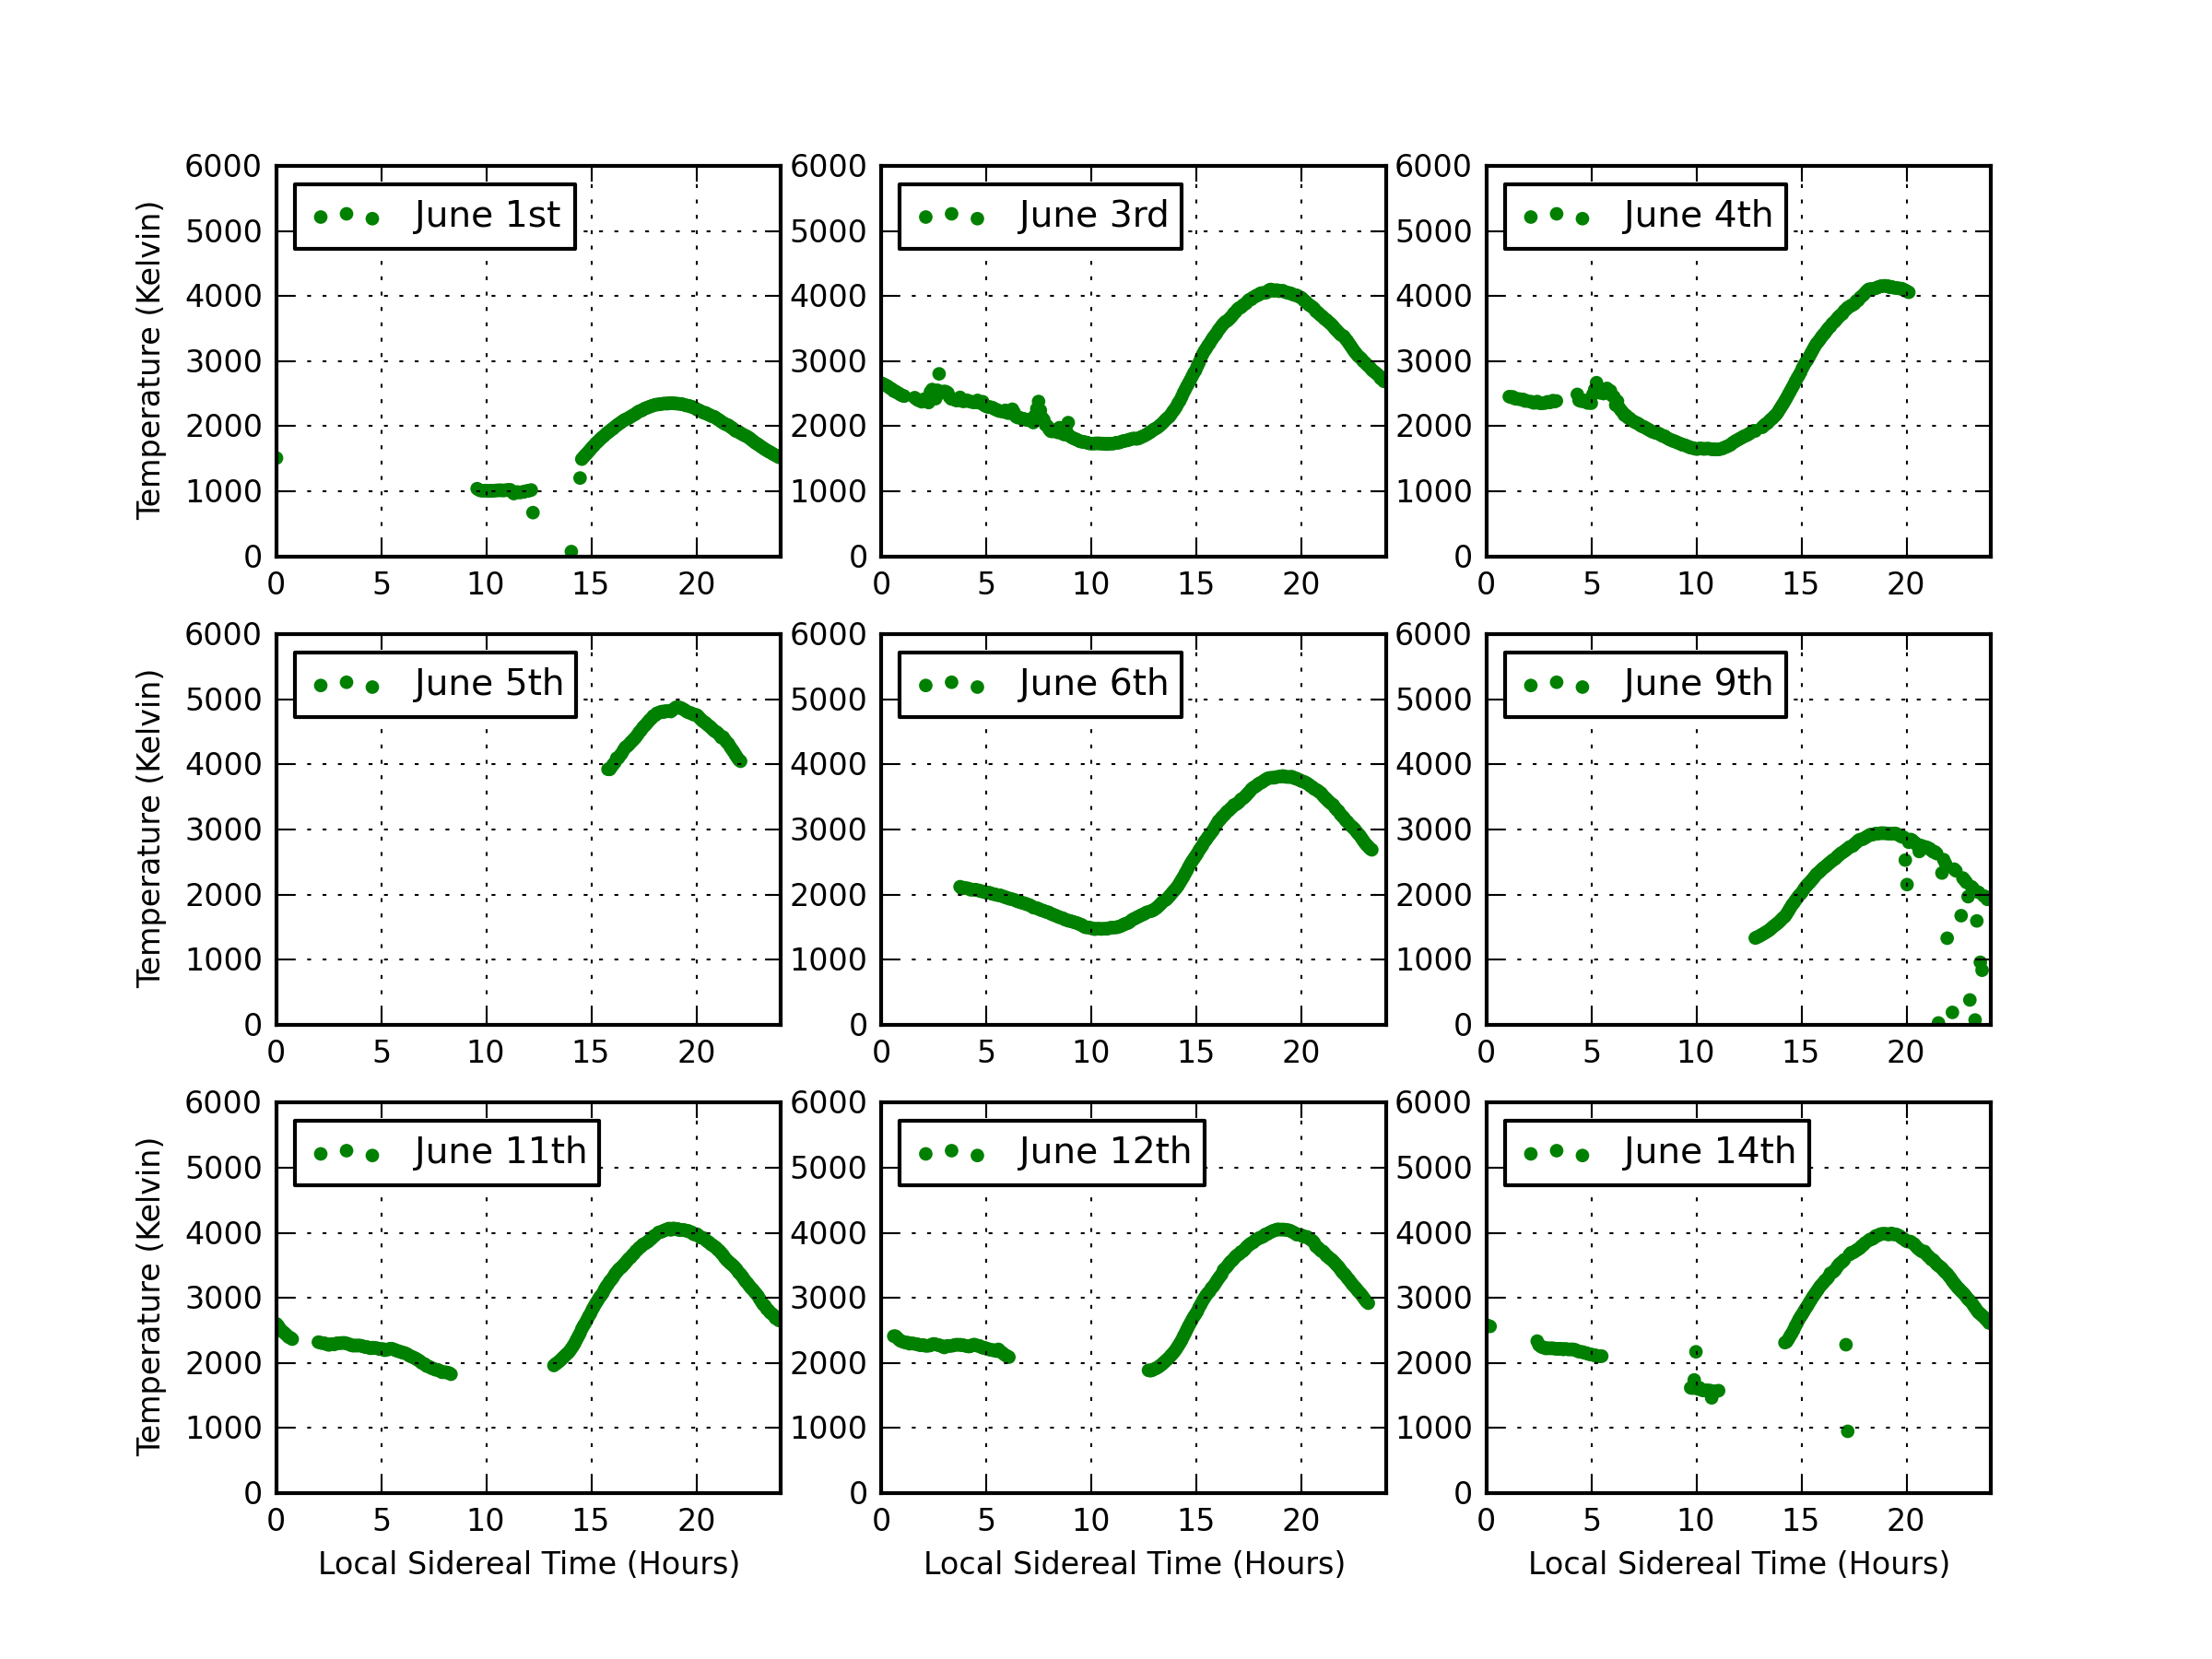
\includegraphics[width=0.95\linewidth]{Data_analysis/figures/Combined_Kdgsm_time_series.png}
\caption{Fits for $K_{\Delta GSM}$ calibration term for multiple days in June 2013 at 70 MHz. Days where a smaller percentage of the data is available have poorer fits. }
\label{Fig:Kdgsm_var}
\end{center}
\end{figure}


\subsubsection{Daily Variance with GSM Modelling}

An alternative to calibration using the Johnson noise datasets is calibration using a source on the sky, which in our case is the Milky Way Galaxy. 

From our GSM model, we have an equation for the sky temperature ($T_{GSM}$), so our $P_{sky}$ can be calculated as:

\begin{equation}
P_{sky} = K_{\Delta GSM}*T_{sky} = K_{\Delta GSM} * T_{GSM}
\end{equation}

And $K_{\Delta GSM}$ can be calculated using:

\begin{equation}
K_{\Delta GSM} = \frac{T_{GSM}}{P_{sky}} = \frac{T_{GSM}* \eta}{P_{ant}-P_{short}}
\end{equation}

In order to maximize the accuracy of $T_{GSM}$, it is better to use the combination of data from a full sidereal day rather than a single time step and remove the time independent component of the data. A $\chi^2$ fitting can then be done  for each frequency independently to get a $K_{\Delta GSM}$ value for that frequency. The $\chi^2$ fit can be written as:

\begin{equation}
\chi^2(\nu) =  \sum_t \big [ \Delta T_{sky}(\nu,t) - \Delta T_{GSM}(\nu,t) \big ]^2
\end{equation}

where $\Delta T_{sky} (\nu, t) = T_{sky}(\nu,t)-\langle T_{sky} \rangle_{DAY} (\nu)$ and $\Delta T_{GSM} (\nu,t) = T_{GSM}(\nu,t)-\langle T_{GSM} \rangle_{DAY} (\nu)$. 

This calibration strategy can be considered analogous to the traditional radio calibration strategy, where the telescope points on and off the source. Once the fit has been calculated, it can be applied to the data (as shown in Figure \ref{Fig:Kdgsm}). 


In order for this calibration strategy to be successful, it is necessary to have the full day of data. When the calibration strategy is applied to a dataset where less than a full day of data is available, inaccuracies in the simulated beam or GSM model have a larger impact on the calibration. This can be seen in Figure \ref{Fig:Kdgsm_var}, where the magnitude of $K_{\Delta GSM}$ at a particular frequency is clearly different when less of the day's data is available. 

\section{Removing the Foregrounds}

\textcolor{red}{Add figure that shows the data before/after foreground removal for one day of data. Have to decide which of the calibration strategies to show...}

\subsection{Polynomial Fitting}
Once the data has been calibrated, the Milky Way Galaxy and other foregrounds have to be removed to reveal the \cm structure. This removal is possible thanks to the simplicity of the galactic sky-averaged brightness temperature ($T_{GM}(\nu)$). 

\begin{equation}
T_{GM}(\nu) = \langle T_{sky}(\nu,t) \rangle_{DAY} - T_{\cm} (\nu) - T_{resid} (\nu)
\end{equation}

We can model $T_{GM} (\nu)$ as a simple polynomial of the form:

\begin{equation}
log_{10} T_{GM}(\nu) = \sum_{k=0}^n a_k \Big[ log_{10} \Big(\frac{\nu}{70 MHz}\Big) \Big]^k
\end{equation}

A n=2 polynomial captures the band average expected foreground brightness temperature ($a_0$), a power law spectral shape ($a_1$), and a synchrotron self-absorption correction term ($a_2$). Once we subtract this polynomial, we are left with residuals:

\begin{equation}
\Delta T (\nu) = T_{\cm}(\nu)+T_{resid}(\nu)
\end{equation}

\begin{figure}[htb]
\begin{center}
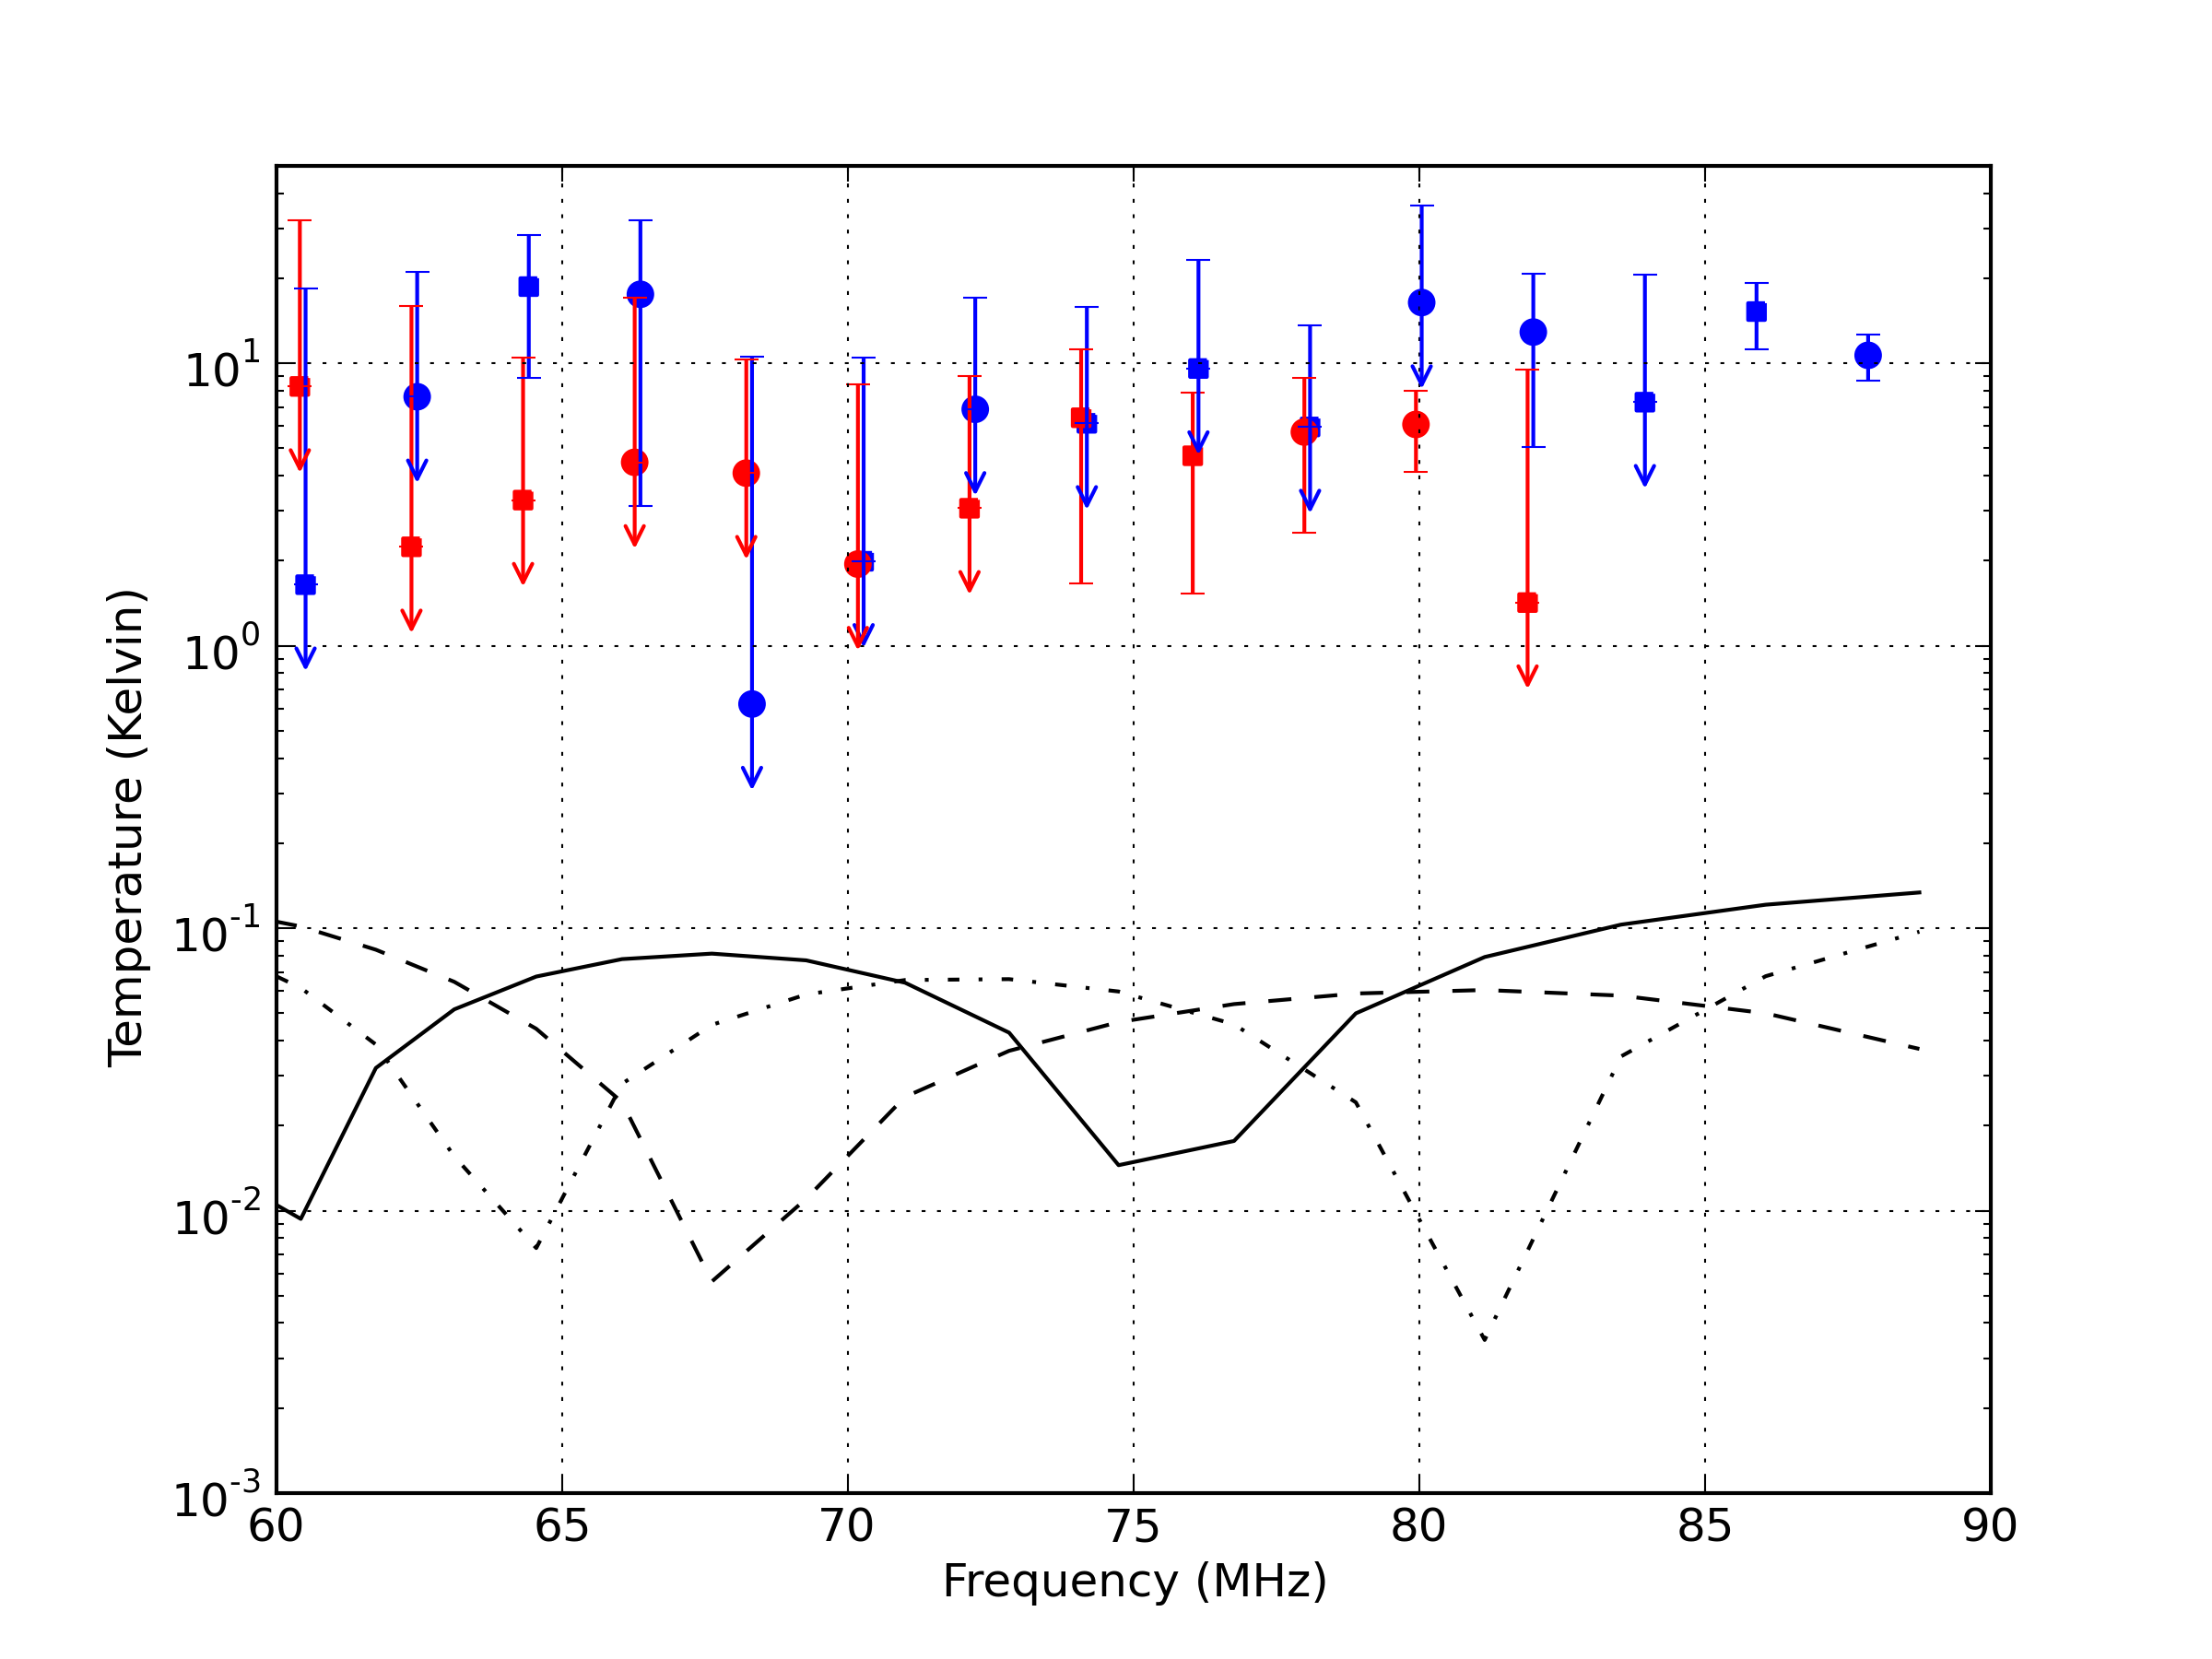
\includegraphics[width=0.95\linewidth]{Data_analysis/figures/joint_log_means.png}
\caption{Daily residuals and variance for data calibrated using either the Galaxy calibration (red) or Johnson Noise calibration (blue) compared to different models of the \cm signal (black). }
\label{Fig:resid}
\end{center}
\end{figure}

\subsection{Daily Residuals}
This fit can be applied separately for each daily mean, giving a distribution of data at each frequency. If $T_{resid}(\nu)$ is significantly smaller than $T_{\cm}$, then a measurement of the \cm structure can be made. The distributions of the daily residuals from the June 2013 for different calibration strategies are shown in Figure \ref{Fig:resid}. These results were first published in the SCI-HI paper \cite{Voytek_2014}.  

\subsection{Frequency Limitations}
In order to achieve reasonable residuals, it was necessary to limit the frequency range of the analysis to avoid frequencies where $T_{resid}$ is large due to RFI from the SCI-HI system or other external sources. In the data collected in June 2013, the useable frequencies were limited to $\sim 60-85 MHz$. Below 60 MHz, there was additional large scale structure in the spectra, which may be due to either ionospheric impacts on the beam shape or inaccuracies in the simulated HIbiscus beam compared to the actual beam. Above 85 MHz there was contamination from both external FM signals and self-generated noise. 

\begin{figure}[htb]
\begin{center}
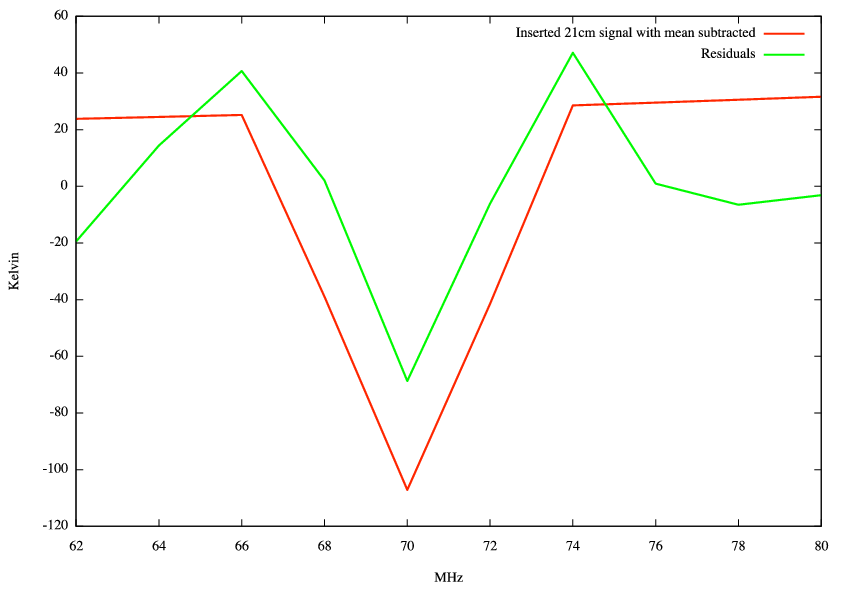
\includegraphics[width=0.9\linewidth]{Data_analysis/figures/100_K_21cm_signal.png}
\caption{Simulated \cm signal with 100 K magnitude (red) and residuals (green) ater calibration and foreground removal. }
\label{Fig:100K_sim}
\end{center}
\end{figure}

\section{\cm Signal Attenuation}
An important cross-check for any \cm measurement experiment is a simulation calibration measurement of signal attenuation \cite{paciga_2013}. This check is done by adding a simulated \cm signal to the raw data and then running the combination data through the signal pipeline. Figure \ref{Fig:100K_sim} shows what happens when a simulated \cm signal, magnified to 100 K to make it easy to identify, is run through the analysis pipeline. 

Because the \cm signal is constant with time, there is minimal signal attenuation caused by the calibration strategy and foreground removal. 


